\PassOptionsToPackage{unicode}{hyperref}
\documentclass[aspectratio=1610, 9pt]{beamer}

% Load packages you need here
%\usepackage{polyglossia}
%\setmainlanguage{german}

\usepackage{csquotes}

\usepackage{amsmath}
\usepackage{amssymb}
\usepackage{mathtools}

\usepackage{braket}
\usepackage{graphicx}

\usepackage{hyperref}
\hypersetup{
  linkcolor= {tudark}, % internal links
  citecolor={tugreen}, % citations
  urlcolor={tudark} % external links/urls
  }
\usepackage{bookmark}
\usepackage{subcaption}
\usepackage[english]{babel}
\usepackage[
backend=biber,
style=authoryear-comp
]{biblatex}

\bibliography{lit.bib}

\usepackage{siunitx}
\usepackage{multicol}

\usepackage{booktabs}

\definecolor{light-gray}{HTML}{b0b5b0}

% load the theme after all packages

\usetheme[
  showtotalframes, % show total number of frames in the footline
]{tudo}

% Put settings here, like
\unimathsetup{
  math-style=ISO,
  bold-style=ISO,
  nabla=upright,
  partial=upright,
  mathrm=sym,
}

\title{Sprechstunde zu:\\Klassifikation von Tiergesichtern in drei Kategorien}
\author[T.~Magorsch,~J.~L.~Späh]{Tom Magorsch\\ Jan Lukas Späh}
\institute[ML-Seminar]{\\[0.3cm]TU Dortmund \\ \Large ML-Seminar}

\begin{document}

\maketitle


\begin{frame}{Erinnerung: Fragestellung und Datensatz}

  \begin{columns}
    \column{0.8\textwidth}
    \begin{itemize}
      \item Klassfikationsproblem: Hund, Katze, Wildtier\\
      \item $16130$ farbige Bilder verschiedener Tiere: $512\times 512$ Pixel
    \end{itemize}
    \column{0.2\textwidth}
    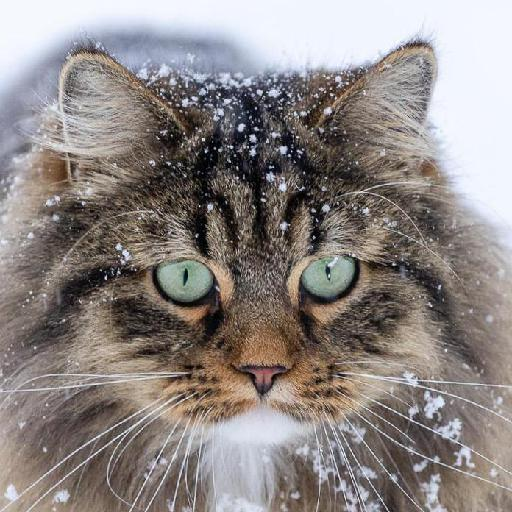
\includegraphics[scale=0.13]{images/cat.jpg}\\
    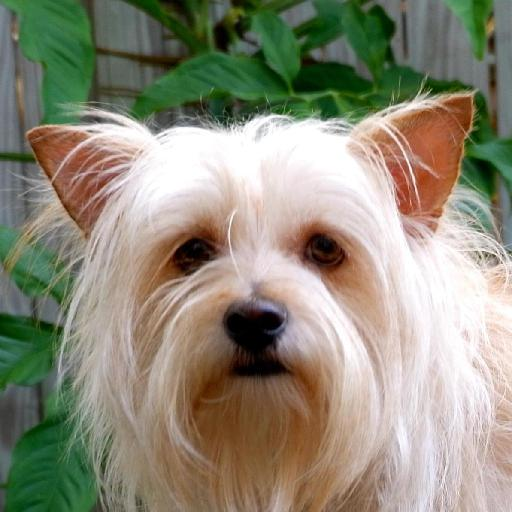
\includegraphics[scale=0.13]{images/dog.jpg}\\
    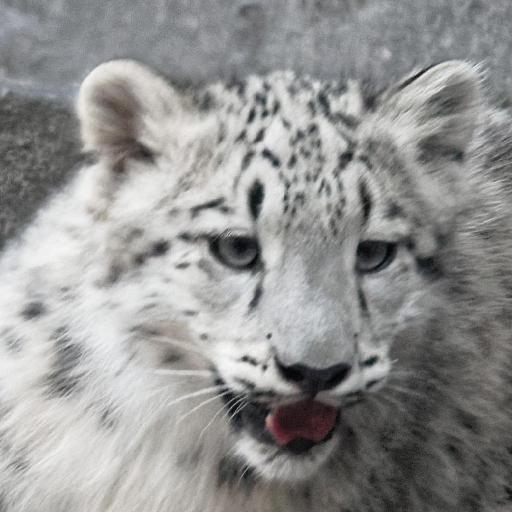
\includegraphics[scale=0.13]{images/wildlife.jpg}\\
  \end{columns}

\end{frame}

\begin{frame}{Training der Daten}
  \begin{itemize}
  \item \textbf{Problem:} Rohdaten passen nicht in den Arbeitsspeicher.
  \item \textbf{Lösung:} Lade Daten während dem Training in Batches in den RAM
    \begin{enumerate}
    \item Lade Bilder mit imread während dem Training
    \item Erstelle .h5 und lade Bilder daraus
    \end{enumerate}
  \item Training mit Data Generator jedoch langsamer
  \item Test mit 1200 training und 300 validation Bilder - 50 Mio Parameter:
    \begin{enumerate}
    \item Training mit Bildern im RAM: 261s
    \item Training mit imgread: 338s
    \item Training mit h5: 318s
    \end{enumerate}
  \end{itemize}
  \centering
  \LARGE
  \textbf{Frage:} Ist Methode 1. eine geeignete Methode oder gibt es bessere Alternativen?
\end{frame}


\begin{frame}{DNN vs CNN}
  \begin{itemize}
  \item Zwei Netzwerke die prinzipiell funktionieren.
  \item Nächster Schritt: Hyperparameter Optimierung
  \end{itemize}

  \begin{figure}
    \centering
    \begin{subfigure}{0.4\textwidth}
      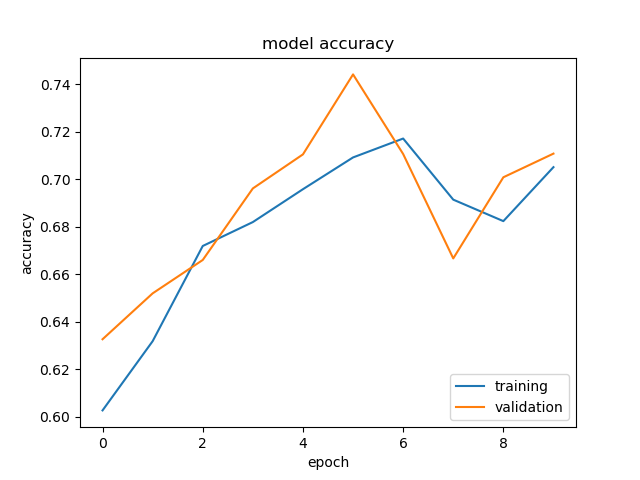
\includegraphics[scale=0.35]{images/dnn_acc2.png}
      \caption{Accuracy des DNN}
      \label{fig:dnn}
    \end{subfigure}
    \begin{subfigure}{0.4\textwidth}
      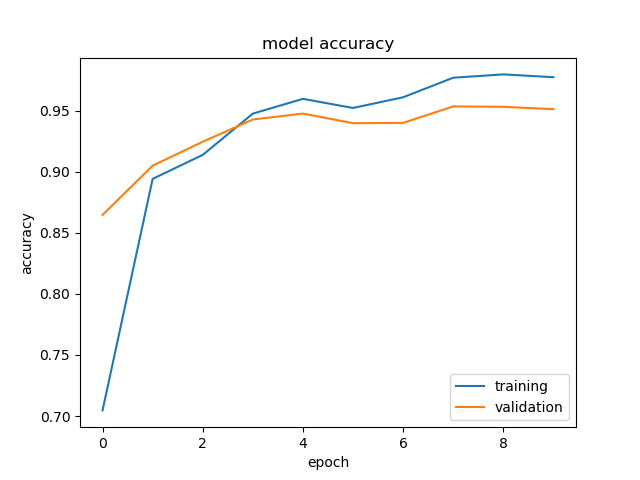
\includegraphics[scale=0.35]{images/cnn_acc.png}
      \caption{Accuracy des CNN}
      \label{fig:cnn}
    \end{subfigure}
  \end{figure}

\end{frame}

\begin{frame}{Alternativmethode}

  \begin{itemize}
    \item Alternativmethode als Benchmark/Motivation für anspruchsvollere Methoden (hier: CNN)
    \item \textbf{Idee:} kNN-Classifier mit reinen Pixelwerten
    \begin{itemize}
      \item Vorteil: Einfach und schafft Klassfikation mit ca. 50\% Accuracy
      \item \textbf{Problem:} Speicherintensiv. Muss im Prinzip alle Trainingsdaten im RAM haben
    \end{itemize}
    \item \textbf{Frage:} Wie diesen Nachteil lösen oder umgehen?? Möglichkeiten:
    \begin{itemize}
      \item Bilder iterativ downscalen und damit arbeiten
      \item Datensatz aufteilen in $n$ Häppchen, die in RAM passen, kNN fitten und evaluieren mit angemessen val\_split\\
      \rightarrow{} Erhalte val\_acc auf komplettem Datensatz mit Unsicherheit
    \end{itemize}
    %\item Zweite Idee: PCA $\to$ SVM, BDT oder Ähnliches
    %\item Es existieren Methoden, PCA inkrementell zu machen. Alternativ: PCA berechnen in Colab, abspeichern und laden
  \end{itemize}

\end{frame}


\begin{frame}{Ideen zum Ausbau des Projekts}

  \begin{itemize}
    \item Zusammenfassend: Erste Alternativmethode funktioniert schlechter als bereits zufriedenstellendes CNN
    \item \textbf{Frage:} Welche weiteren Schritte?
    \begin{itemize}
      \item Sequentielle Hyperparametersuche für kNN und Netze
      \item Bestes Netz aufschneiden und Output einer Lage clustern\\
      \rightarrow{} Von Hand inspizieren. Sind Tierarten oder Muster erkennbar (Wild)?
      %s\item Einfall: Klassischen Hund/Katze Datensatz und Performance testen.
      \item Auch möglich: Wähle selbst Bilder bestimmter Arten aus und interpretiere Output
    \end{itemize}
    \item \textbf{Frage:} Guter Plan? Ab wo ausreichend für das Projekt?
  \end{itemize}

\end{frame}



\end{document}
